\documentclass[11pt,preprint, authoryear]{elsarticle}

\usepackage{lmodern}
%%%% My spacing
\usepackage{setspace}
\setstretch{1.2}
\DeclareMathSizes{12}{14}{10}{10}

% Wrap around which gives all figures included the [H] command, or places it "here". This can be tedious to code in Rmarkdown.
\usepackage{float}
\let\origfigure\figure
\let\endorigfigure\endfigure
\renewenvironment{figure}[1][2] {
    \expandafter\origfigure\expandafter[H]
} {
    \endorigfigure
}

\let\origtable\table
\let\endorigtable\endtable
\renewenvironment{table}[1][2] {
    \expandafter\origtable\expandafter[H]
} {
    \endorigtable
}


\usepackage{ifxetex,ifluatex}
\usepackage{fixltx2e} % provides \textsubscript
\ifnum 0\ifxetex 1\fi\ifluatex 1\fi=0 % if pdftex
  \usepackage[T1]{fontenc}
  \usepackage[utf8]{inputenc}
\else % if luatex or xelatex
  \ifxetex
    \usepackage{mathspec}
    \usepackage{xltxtra,xunicode}
  \else
    \usepackage{fontspec}
  \fi
  \defaultfontfeatures{Mapping=tex-text,Scale=MatchLowercase}
  \newcommand{\euro}{€}
\fi

\usepackage{amssymb, amsmath, amsthm, amsfonts}

\def\bibsection{\section*{References}} %%% Make "References" appear before bibliography


\usepackage[round]{natbib}

\usepackage{longtable}
\usepackage[margin=2.3cm,bottom=2cm,top=2.5cm, includefoot]{geometry}
\usepackage{fancyhdr}
\usepackage[bottom, hang, flushmargin]{footmisc}
\usepackage{graphicx}
\numberwithin{equation}{section}
\numberwithin{figure}{section}
\numberwithin{table}{section}
\setlength{\parindent}{0cm}
\setlength{\parskip}{1.3ex plus 0.5ex minus 0.3ex}
\usepackage{textcomp}
\renewcommand{\headrulewidth}{0.2pt}
\renewcommand{\footrulewidth}{0.3pt}

\usepackage{array}
\newcolumntype{x}[1]{>{\centering\arraybackslash\hspace{0pt}}p{#1}}

%%%%  Remove the "preprint submitted to" part. Don't worry about this either, it just looks better without it:
\makeatletter
\def\ps@pprintTitle{%
  \let\@oddhead\@empty
  \let\@evenhead\@empty
  \let\@oddfoot\@empty
  \let\@evenfoot\@oddfoot
}
\makeatother

 \def\tightlist{} % This allows for subbullets!

\usepackage{hyperref}
\hypersetup{breaklinks=true,
            bookmarks=true,
            colorlinks=true,
            citecolor=blue,
            urlcolor=blue,
            linkcolor=blue,
            pdfborder={0 0 0}}


% The following packages allow huxtable to work:
\usepackage{siunitx}
\usepackage{multirow}
\usepackage{hhline}
\usepackage{calc}
\usepackage{tabularx}
\usepackage{booktabs}
\usepackage{caption}


\newenvironment{columns}[1][]{}{}

\newenvironment{column}[1]{\begin{minipage}{#1}\ignorespaces}{%
\end{minipage}
\ifhmode\unskip\fi
\aftergroup\useignorespacesandallpars}

\def\useignorespacesandallpars#1\ignorespaces\fi{%
#1\fi\ignorespacesandallpars}

\makeatletter
\def\ignorespacesandallpars{%
  \@ifnextchar\par
    {\expandafter\ignorespacesandallpars\@gobble}%
    {}%
}
\makeatother

\newlength{\cslhangindent}
\setlength{\cslhangindent}{1.5em}
\newenvironment{CSLReferences}%
  {\setlength{\parindent}{0pt}%
  \everypar{\setlength{\hangindent}{\cslhangindent}}\ignorespaces}%
  {\par}


\urlstyle{same}  % don't use monospace font for urls
\setlength{\parindent}{0pt}
\setlength{\parskip}{6pt plus 2pt minus 1pt}
\setlength{\emergencystretch}{3em}  % prevent overfull lines
\setcounter{secnumdepth}{5}

%%% Use protect on footnotes to avoid problems with footnotes in titles
\let\rmarkdownfootnote\footnote%
\def\footnote{\protect\rmarkdownfootnote}
\IfFileExists{upquote.sty}{\usepackage{upquote}}{}

%%% Include extra packages specified by user

%%% Hard setting column skips for reports - this ensures greater consistency and control over the length settings in the document.
%% page layout
%% paragraphs
\setlength{\baselineskip}{12pt plus 0pt minus 0pt}
\setlength{\parskip}{12pt plus 0pt minus 0pt}
\setlength{\parindent}{0pt plus 0pt minus 0pt}
%% floats
\setlength{\floatsep}{12pt plus 0 pt minus 0pt}
\setlength{\textfloatsep}{20pt plus 0pt minus 0pt}
\setlength{\intextsep}{14pt plus 0pt minus 0pt}
\setlength{\dbltextfloatsep}{20pt plus 0pt minus 0pt}
\setlength{\dblfloatsep}{14pt plus 0pt minus 0pt}
%% maths
\setlength{\abovedisplayskip}{12pt plus 0pt minus 0pt}
\setlength{\belowdisplayskip}{12pt plus 0pt minus 0pt}
%% lists
\setlength{\topsep}{10pt plus 0pt minus 0pt}
\setlength{\partopsep}{3pt plus 0pt minus 0pt}
\setlength{\itemsep}{5pt plus 0pt minus 0pt}
\setlength{\labelsep}{8mm plus 0mm minus 0mm}
\setlength{\parsep}{\the\parskip}
\setlength{\listparindent}{\the\parindent}
%% verbatim
\setlength{\fboxsep}{5pt plus 0pt minus 0pt}



\begin{document}



\begin{frontmatter}  %

\title{Question 2}

% Set to FALSE if wanting to remove title (for submission)




\author[Add1]{Joshua Strydom\footnote{\textbf{Contributions:}
  \newline \emph{The authors would like to thank no institution for
  money donated to this project. Thank you sincerely.}}}
\ead{20718284@sun.ac.za}





\address[Add1]{Stellenbosch University, Stellenbosch, South Africa}



\vspace{1cm}





\vspace{0.5cm}

\end{frontmatter}



%________________________
% Header and Footers
%%%%%%%%%%%%%%%%%%%%%%%%%%%%%%%%%
\pagestyle{fancy}
\chead{}
\rhead{}
\lfoot{}
\rfoot{\footnotesize Page \thepage}
\lhead{}
%\rfoot{\footnotesize Page \thepage } % "e.g. Page 2"
\cfoot{}

%\setlength\headheight{30pt}
%%%%%%%%%%%%%%%%%%%%%%%%%%%%%%%%%
%________________________

\headsep 35pt % So that header does not go over title




\hypertarget{yield-spreads}{%
\section{\texorpdfstring{Yield spreads
\label{Yield}}{Yield spreads }}\label{yield-spreads}}

\begin{figure}[H]

{\centering \includegraphics{Question2_files/figure-latex/Figure1-1} 

}

\caption{Caption Here \label{Figure1}}\label{fig:Figure1}
\end{figure}

The bond spread has over time increased but it is by no means high
compared to historical spreads.

\begin{figure}[H]

{\centering \includegraphics{Question2_files/figure-latex/Figure2-1} 

}

\caption{Caption Here \label{Figure2}}\label{fig:Figure2}
\end{figure}

The bond spread has, over time, gradually increased. The yield spread
between the 2 year and 10 year bonds have, since 2020, been the highest
in decades.

\begin{figure}[H]

{\centering \includegraphics{Question2_files/figure-latex/Figure3-1} 

}

\caption{Caption Here \label{Figure3}}\label{fig:Figure3}
\end{figure}

The bond spread has, over time, gradually increased. The yield spread
between the 3 month and 10 year bonds have, since 2020, been the highest
in decades.

\begin{figure}[H]

{\centering \includegraphics{Question2_files/figure-latex/Figure4-1} 

}

\caption{Caption Here \label{Figure4}}\label{fig:Figure4}
\end{figure}

One can clearly see, from Figure \ref{Figure4}, that all of the yield
spreads become far larger from 2020 from an historical context. The
spread between the 3 month and 10 year bonds as well as the spread
between the 2 year and 10 year bonds are greatest during this respective
period. The spreads seemed to have followed each others movements
closely for the whole period.

\hypertarget{comparing-yields-of-international-counterparts}{%
\section{\texorpdfstring{Comparing yields of international counterparts
\label{International}}{Comparing yields of international counterparts }}\label{comparing-yields-of-international-counterparts}}

\begin{figure}[H]

{\centering \includegraphics{Question2_files/figure-latex/Figure5-1} 

}

\caption{Caption Here \label{Figure5}}\label{fig:Figure5}
\end{figure}

The Nigerian 2 year bond yield appears to be highest with Russia's being
second largest. The South African 2 year bond yield ranks third highest
out of the group. The Euro 2 year bond yield has been consistently
negative from about 2015. If market participants believe that there is
higher inflation on the horizon, interest rates and bond yields will
rise (and prices will decrease) to compensate for the loss of the
purchasing power of future cash flows. Bonds with the longest cash flows
will see their yields rise and prices fall the most.

\begin{figure}[H]

{\centering \includegraphics{Question2_files/figure-latex/Figure6-1} 

}

\caption{Caption Here \label{Figure6}}\label{fig:Figure6}
\end{figure}

The Nigerian 10 year bond yield again appears to be highest while the
South African 10 year yield ranks second this time from 2019 onwards.
The Russian 10 year bond yield ranks approximately third highest out of
the group although dipping below the Indian 10 year bond yield for a
short period (between 2020 and 2021). The Euro 10 year bond yield has
been consistently the lowest for the entire sample period and turned
negative in the 2019 year.

\hypertarget{background-information}{%
\section{\texorpdfstring{Background information
\label{Background}}{Background information }}\label{background-information}}

\begin{figure}[H]

{\centering 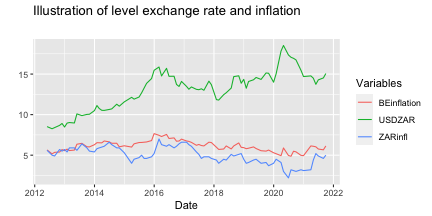
\includegraphics{Question2_files/figure-latex/Figure7-1} 

}

\caption{Caption Here \label{Figure7}}\label{fig:Figure7}
\end{figure}

Actual inflation in South Africa has remained consistently below
breakeven inflation since 2015. The Rand, as can be seen in the large
spike post-2020, weakened against the Dollar. It has since gradually
strengthened but is still high when compared to 10 years ago in 2012.
The increase in South African inflation could explain the fact that bond
yields have increased recently. Bonds yields would've risen primarily
because of a hawkish position of the SARB. Investors thus anticipate
aggressive interest rate hikes to rein in inflation.

\begin{figure}[H]

{\centering \includegraphics{Question2_files/figure-latex/Figure8-1} 

}

\caption{Caption Here \label{Figure8}}\label{fig:Figure8}
\end{figure}

The graph above depicts the change (calculated the same as a simple
return) of the South African inflation rate. It is easy to tell that the
inflation rate has proven to be more volatile post-2020 than has been
the case historically.

\begin{figure}[H]

{\centering 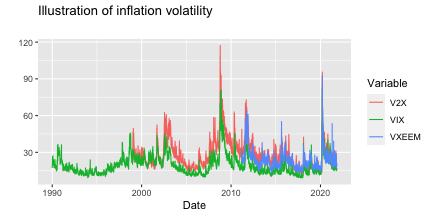
\includegraphics{Question2_files/figure-latex/Figure9-1} 

}

\caption{Caption Here \label{Figure9}}\label{fig:Figure9}
\end{figure}

Figure \ref{Figure9} reinterates the point made about Figure
\ref{Figure8}. The largest spike in inflation volatility occurred in
2009 but this is to be expected. Inflation volatility had since declined
but spiked again in 2020. Increased inflation and the volatility thereof
generally leads to an increase in longer dated bond yields. This would
explain the increase in longer dated bond spreads.

\hypertarget{conclusion}{%
\section{Conclusion}\label{conclusion}}

Yield spread in local mid to longer dated bond yields have since 2020
been the highest in decades.

\bibliography{Tex/ref}





\end{document}
